\documentclass[10pt,aspectratio=169]{beamer}

%================================================
% Theme
%================================================
\usetheme[numbering=fraction,progressbar=frametitle]{metropolis}
\metroset{block=fill}

%================================================
% Packages
%================================================
\usepackage{amsmath,amssymb}
\usepackage{booktabs}
\usepackage{xcolor}
\usepackage{listings}
\usepackage{tikz}
\usepackage[useregional,lastcompiled]{datetime2}
\usetikzlibrary{positioning,arrows.meta,shapes.misc,fit}

%================================================
% Version macro
%================================================
%\newcommand{\LastEditVersion}{v0.2 -- 16 June 2026}
\newcommand{\CourseTitle}{Theory of Computation}
\newcommand{\LectureTitle}{Lecture 1: Can Intelligent Machines Compute Everything?}
\newcommand{\LastCompiledTime}{\DTMnow}

%================================================
% Metadata
%================================================
\title{\CourseTitle}
\subtitle{\LectureTitle}
\author{Sheikh Azizul Hakim\\Lecturer, Department of CSE, BUET}
\date{Last compiled: \LastCompiledTime}

%================================================
% Colors
%================================================
\definecolor{tocblue}{HTML}{2457A6}
\definecolor{tocgreen}{HTML}{1B7F5A}
\definecolor{tocorange}{HTML}{C65F21}
\definecolor{tocred}{HTML}{B3261E}
\definecolor{tocpurple}{HTML}{6C3BAA}
\definecolor{softgray}{HTML}{F4F6F8}

\setbeamercolor{alerted text}{fg=tocorange}
\setbeamercolor{block title}{fg=white,bg=tocblue}
\setbeamercolor{block body}{fg=black,bg=softgray}

%================================================
% Code style
%================================================
\lstdefinestyle{code}{
  basicstyle=\ttfamily\small,
  backgroundcolor=\color{black!4},
  frame=single,
  rulecolor=\color{black!18},
  columns=fullflexible,
  keepspaces=true,
  showstringspaces=false,
  breaklines=true
}
\lstset{style=code}

%================================================
% Small helper commands
%================================================
\newcommand{\BigQ}[1]{\begin{center}\Large\bfseries #1\end{center}}
\newcommand{\tagline}[1]{\begin{center}\alert{#1}\end{center}}

%================================================
\begin{document}

%------------------------------------------------
\maketitle

%------------------------------------------------
\begin{frame}[standout]
This course is not about old machines.

\vspace{1em}
It is about the limits of \alert{all} machines.
\end{frame}

%------------------------------------------------
\begin{frame}[fragile]{Four Things That Look Easy}
\begin{columns}[T,totalwidth=\textwidth]
\column{0.48\textwidth}
\textbf{1. Parentheses}
\begin{lstlisting}
(((((((((((((())))))))))))))
\end{lstlisting}

\vspace{0.7em}
\textbf{2. JSON}
\begin{lstlisting}
{
  "students": [
    { "name": "Rahim",
      "courses": ["CSE", "EEE"] }
  ]
}
\end{lstlisting}

\column{0.48\textwidth}
\textbf{3. Program behavior}
\begin{lstlisting}
while True:
    pass
\end{lstlisting}

\vspace{0.7em}
\textbf{4. Sudoku}
\begin{lstlisting}
Given a filled board: check it.
Given an empty puzzle: solve it.
\end{lstlisting}
\end{columns}

\pause
\vspace{0.5em}
\tagline{These four examples motivate almost the entire course.}
\end{frame}

%------------------------------------------------
\begin{frame}{Prediction Game}
Before learning the theory, guess the answer.

\vspace{0.7em}
\begin{center}
\begin{tabular}{lll}
\toprule
\textbf{Problem} & \textbf{Solvable?} & \textbf{Efficient?} \\
\midrule
Check password rules & ? & ? \\
Check balanced parentheses & ? & ? \\
Validate JSON & ? & ? \\
Predict whether any program halts & ? & ? \\
Solve arbitrary Sudoku & ? & ? \\
Perfectly verify AI-generated code & ? & ? \\
\bottomrule
\end{tabular}
\end{center}

\pause
\vspace{0.5em}
\tagline{We will revisit this table throughout the semester.}
\end{frame}

%------------------------------------------------
\begin{frame}{The Four Mysteries}
\begin{block}{Mystery 1}
Can finite memory understand arbitrarily deep structure?
\end{block}

\begin{block}{Mystery 2}
Can every problem be solved algorithmically?
\end{block}

\begin{block}{Mystery 3}
Can every program be analyzed automatically?
\end{block}

\begin{block}{Mystery 4}
Can every efficiently checkable solution also be efficiently found?
\end{block}
\end{frame}

%------------------------------------------------
\begin{frame}[fragile]{Mystery 1: Password Rules}
A website asks for a password:

\begin{lstlisting}
At least 8 characters
Contains a digit
Contains an uppercase letter
Contains no spaces
\end{lstlisting}

\pause
\begin{columns}[T]
\column{0.48\textwidth}
\begin{lstlisting}
Abcdef12     valid
A1bcdefg     valid
\end{lstlisting}

\column{0.48\textwidth}
\begin{lstlisting}
abcdef12     invalid
ABC DEF12    invalid
\end{lstlisting}
\end{columns}

\pause
\vspace{0.8em}
\BigQ{How much memory is needed?}

\pause
\tagline{Only finite memory. This leads to finite automata.}
\end{frame}

%------------------------------------------------
\begin{frame}[fragile]{Mystery 1: Tokenizing Code}
Your compiler sees this:

\begin{lstlisting}
if (x == 10) return x + 1;
\end{lstlisting}

\pause
But internally it may see this:

\begin{lstlisting}
IF LPAREN ID EQEQ NUM RPAREN RETURN ID PLUS NUM SEMICOLON
\end{lstlisting}

\pause
\vspace{0.8em}
\BigQ{How does raw text become structure?}

\pause
\tagline{Regular expressions, DFA, and NFA are behind this story.}
\end{frame}

%------------------------------------------------
\begin{frame}[fragile]{But Finite Memory Hits a Wall}
Balanced:
\begin{lstlisting}
()
(())
((()))
(()(()))
\end{lstlisting}

\pause
Not balanced:
\begin{lstlisting}
(()))(
(((
())(()
\end{lstlisting}

\pause
\vspace{0.6em}
\BigQ{Can finite memory handle arbitrary nesting?}

\pause
\tagline{No. We need stronger models.}
\end{frame}

%------------------------------------------------
\begin{frame}[fragile]{Mystery 2: Why VS Code Knows Something Is Missing}
Incomplete JSON:

\begin{lstlisting}
{
  "students": [
    {
      "name": "Rahim",
      "courses": ["CSE", "EEE"]
\end{lstlisting}

\pause
\BigQ{What is the editor remembering?}

\pause
\vspace{0.5em}
It remembers what still needs to be closed:

\begin{center}
\large
\texttt{\{} \quad \texttt{[} \quad \texttt{\{} \quad \texttt{[}
\end{center}

\pause
\tagline{This is stack-like memory. This leads to pushdown automata.}
\end{frame}

%------------------------------------------------
\begin{frame}{A Visual Hierarchy of Memory}
\begin{center}
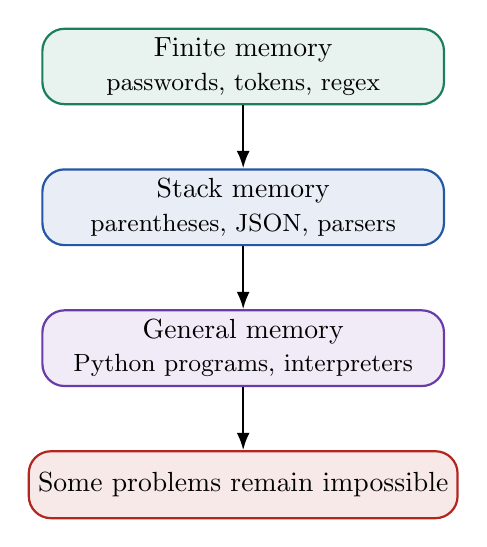
\begin{tikzpicture}[
    node distance=0.8cm,
    box/.style={draw, rounded corners=8pt, minimum width=5.1cm, minimum height=0.85cm, align=center, thick},
    arrow/.style={-{Latex[length=2.2mm]}, thick}
]

\node[box, fill=tocgreen!10, draw=tocgreen] (finite) {Finite memory\\\small passwords, tokens, regex};
\node[box, fill=tocblue!10, draw=tocblue, below=of finite] (stack) {Stack memory\\\small parentheses, JSON, parsers};
\node[box, fill=tocpurple!10, draw=tocpurple, below=of stack] (general) {General memory\\\small Python programs, interpreters};
\node[box, fill=tocred!10, draw=tocred, below=of general] (limits) {Some problems remain impossible};

\draw[arrow] (finite) -- (stack);
\draw[arrow] (stack) -- (general);
\draw[arrow] (general) -- (limits);

\end{tikzpicture}
\end{center}
\end{frame}

%------------------------------------------------
\begin{frame}[fragile]{Mystery 3: Will This Program Stop?}
\begin{columns}[T,totalwidth=\textwidth]
\column{0.48\textwidth}
\textbf{Obviously stops}
\begin{lstlisting}
print("Hello")
\end{lstlisting}

\column{0.48\textwidth}
\textbf{Obviously does not stop}
\begin{lstlisting}
while True:
    pass
\end{lstlisting}
\end{columns}

\pause
\vspace{1em}
But what about an arbitrary program with thousands of lines?

\pause
\vspace{0.8em}
\BigQ{Can we build a perfect halt-detector?}

\pause
\tagline{No. This is not an engineering failure. It is a theorem.}
\end{frame}

%------------------------------------------------
\begin{frame}{A Shocking Theorem Coming Later}
\begin{block}{Halting Problem}
There is no program that can perfectly determine whether every other program eventually halts.
\end{block}

\pause
\vspace{1em}
Consequences:

\begin{itemize}
    \item no perfect bug detector,
    \item no perfect malware detector,
    \item no perfect program verifier for all programs,
    \item no AI system that can bypass this for arbitrary code.
\end{itemize}

\pause
\tagline{Useful tools exist. Perfect tools do not.}
\end{frame}

%------------------------------------------------
\begin{frame}{Mystery 4: Checking vs Finding}
\begin{columns}[T,totalwidth=\textwidth]
\column{0.48\textwidth}
\begin{block}{Checking}
Given a completed Sudoku board, we can quickly check whether it is valid.
\end{block}

\column{0.48\textwidth}
\begin{block}{Finding}
Given an empty or partial puzzle, finding a solution may require enormous search.
\end{block}
\end{columns}

\pause
\vspace{1.5em}
\BigQ{Why is verification often easier than discovery? Or is it?}

\pause
\tagline{This question leads to P, NP, reductions, and NP-completeness.}
\end{frame}

%------------------------------------------------
\begin{frame}{AI Does Not Delete Complexity}
An LLM may help us write a Sudoku solver.

\pause
\vspace{0.8em}
But writing a solver is not the same as magically solving every instance instantly.

\pause
\vspace{1.2em}
\begin{center}
\Large
AI can improve heuristics.\\[0.4em]
AI can guide search.\\[0.4em]
AI can generate code.\\[0.4em]
\alert{But AI does not erase worst-case complexity.}
\end{center}
\end{frame}

%------------------------------------------------
\begin{frame}{Can ChatGPT Prove Every Theorem?}
First question:

\begin{center}
\Large
Can ChatGPT prove every true mathematical theorem?
\end{center}

\pause
Second question:

\begin{center}
\Large
Can it prove every theorem that has a short proof?
\end{center}

\pause
\vspace{1em}
This connects theory of computation to:

\begin{itemize}
    \item proof verification,
    \item automated theorem proving,
    \item Lean and formal mathematics,
    \item computational complexity.
\end{itemize}
\end{frame}

%------------------------------------------------
\begin{frame}{Course Map}
\begin{center}
\begin{tabular}{lll}
\toprule
\textbf{Topic} & \textbf{Core question} & \textbf{Concrete examples} \\
\midrule
DFA/NFA & finite memory & passwords, tokens, regex \\
CFG/PDA & stack memory & JSON, parsers, parentheses \\
Turing machines & computation itself & interpreters, programs \\
Undecidability & impossible problems & halting, verification \\
Complexity & feasible computation & Sudoku, SAT, cryptography \\
\bottomrule
\end{tabular}
\end{center}

\pause
\vspace{1em}
\tagline{The course is about the possible, the impossible, and the feasible.}
\end{frame}

%------------------------------------------------
\begin{frame}{How We Will Use AI in TCS/Mathematics}
We will use AI systems as assistants, not oracles.

\pause
\begin{itemize}
    \item Ask an LLM to design an automaton.
    \item Test it with counterexamples.
    \item Ask for a proof.
    \item Find the hidden gap.
    \item Repair the reasoning formally.
\end{itemize}

\pause
\vspace{1em}
\tagline{A good computer scientist does not merely get answers. A good computer scientist verifies them.}
\end{frame}

%------------------------------------------------
\begin{frame}{Main Reference}
\begin{center}
\Large
\textbf{Michael Sipser}\\[0.3em]
\emph{Introduction to the Theory of Computation}
\end{center}

\pause
\vspace{1.5em}
\begin{center}
These slides are a modern companion to the classical theory.
\end{center}

\pause
\vspace{1em}
\tagline{Sipser gives the rigorous core. We will add modern intuition and AI-era examples.}
\end{frame}

%------------------------------------------------
\begin{frame}{By the End of This Course, You Should Know}
\begin{itemize}
    \item why regular expressions work,
    \item why JSON parsing needs memory,
    \item why some program-analysis tools can never be perfect,
    \item why AI cannot solve every search problem instantly,
    \item why P versus NP is one of the deepest questions in computing.
\end{itemize}

\pause
\vspace{1em}
\begin{center}
\Large
\alert{Theory of Computation is the mathematics of computational limits.}
\end{center}
\end{frame}

%================================================
\begin{frame}{Where Is Theory of Computation Alive Today?\\
Theory Meets Artificial Intelligence}

\begin{columns}[T]

\column{0.48\textwidth}
\textbf{Large Language Models}

\begin{itemize}
\item Why do large models generalize?
\item Why do they hallucinate?
\item Can they reason systematically?
\item What are their computational limits?
\end{itemize}

\column{0.48\textwidth}
\textbf{AI for Mathematics}

\begin{itemize}
\item Automated theorem proving
\item LLMs + Lean/Isabelle/Coq
\item Formal verification of AI-generated code
\item Machine-assisted scientific discovery
\end{itemize}

\end{columns}

\vfill

\begin{center}
\alert{Can intelligence transcend the limits of computation?}
\end{center}

\end{frame}
%================================================

%================================================
\begin{frame}{Where Is Theory of Computation Alive Today?\\
Theory Meets Software and Systems}

\begin{columns}[T]

\column{0.48\textwidth}
\textbf{SAT and SMT Solvers}

\begin{itemize}
\item Software verification
\item Hardware verification
\item Program synthesis
\item Scheduling and planning
\item Security analysis
\end{itemize}

\column{0.48\textwidth}
\textbf{Programming Languages}

\begin{itemize}
\item Compilers
\item Static analyzers
\item Type systems
\item Model checking
\item Automated bug detection
\end{itemize}

\end{columns}

\vfill

\begin{center}
\alert{Can every bug be detected automatically?}
\end{center}

\end{frame}
%================================================

%================================================
\begin{frame}{Where Is Theory of Computation Alive Today?\\
Theory Meets the Future of Computing}

\begin{columns}[T]

\column{0.48\textwidth}
\textbf{Complexity Theory}

\begin{itemize}
\item P versus NP
\item Fine-grained complexity
\item Approximation algorithms
\item Hardness of optimization
\item Cryptographic assumptions
\end{itemize}

\column{0.48\textwidth}
\textbf{Emerging Paradigms}

\begin{itemize}
\item Quantum computing
\item Interactive proofs
\item Zero-knowledge proofs
\item Streaming algorithms
\item Distributed computation
\end{itemize}

\end{columns}

\vfill

\begin{center}
\alert{Which problems remain difficult even for future computers?}
\end{center}

\end{frame}
%================================================

%------------------------------------------------
\begin{frame}[standout]
If intelligence is computation,

\vspace{1em}
what are the limits of intelligence itself?
\end{frame}

%================================================
\end{document}
